\section{Malacology: A Programmable Storage System}

\begin{figure}[tb]
\centering
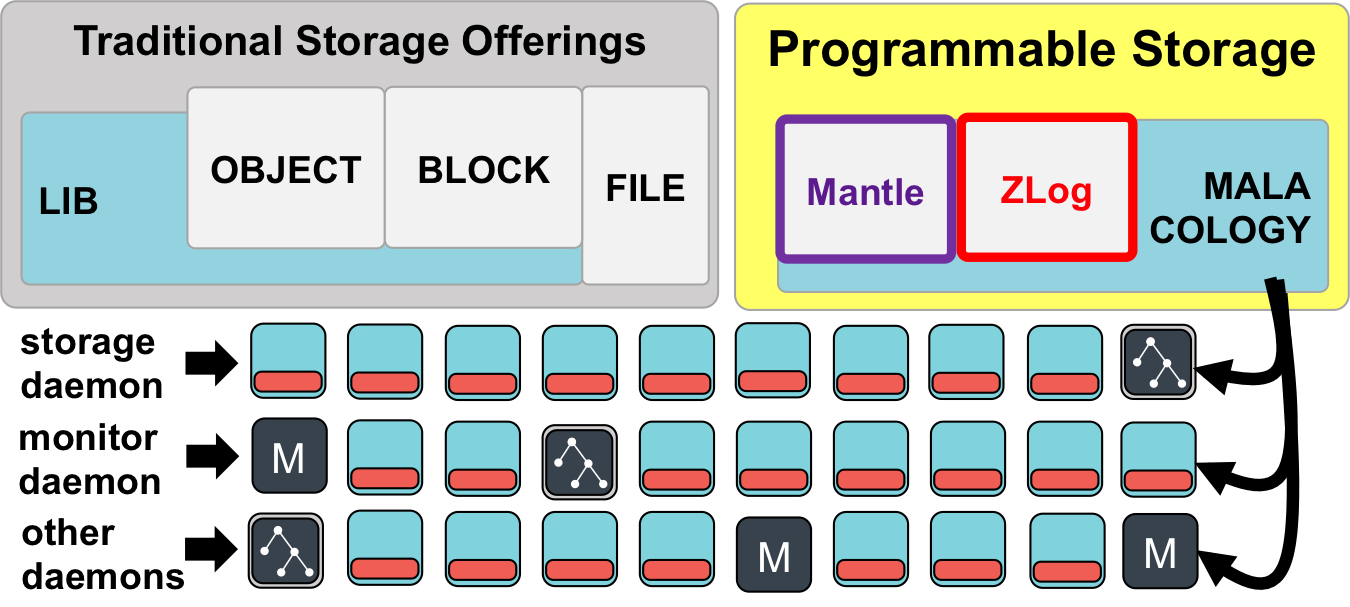
\includegraphics[width=1\textwidth]{./chapters/background/figures/overview.png}
\caption{Scalable storage systems have storage daemons which store data,
monitor daemons (M) that maintain cluster state, and service-specific daemons
(e.g., file system metadata servers). Malacology enables the programmability of
internal abstractions (bold arrows) to re-use and compose existing subsystems.
With Malacology, we built new higher-level services, ZLog and Mantle, that sit
alongside traditional user-facing APIs (file, block,
object).}\label{fig:overview}
\end{figure}

We define a programmable storage system to be a storage system that facilitates
the re-use and extension of existing storage abstractions provided by the
underlying software stack, to enable the creation of new services via
composition.  A programmable storage system can be realized by exposing
existing functionality (such as file system and cluster
metadata services and synchronization and monitoring capabilities) as
interfaces that can be ``glued together'' in a variety of ways using a
high-level language. Programmable storage differs from \emph{active
storage}~\cite{riedel:vldb98}---the injection and execution of code within a
storage system or storage device---in that the former is applicable to any
component of the storage system, while the latter focuses at the data access
level. Given this contrast, we can say that active storage is an example of how
one internal component (the storage layer) is exposed in a programmable storage
system.

To illustrate the benefits and challenges of this approach we have designed and
evaluated Malacology, a programmable storage system that facilitates the
construction of new services by re-purposing existing subsystem abstractions of
the storage stack.  We build Malacology in Ceph, a popular open source software
storage stack.  We choose Ceph to demonstrate the concept of programmable
storage because it offers a broad spectrum of existing services, including
distributed locking and caching services provided by file
system metadata servers, durability and object interfaces provided by the
back-end object store, and propagation of consistent cluster state provided by
the monitoring service (see Figure~\ref{fig:overview}).  Malacology is
expressive enough to provide the functionality necessary for implementing new
services.

Malacology includes a set of interfaces that can be used as
building blocks for constructing novel storage abstractions, including:

\begin{enumerate}

\item An interface for managing strongly-consistent time-varying
\textbf{service metadata}.

\item An interface for installing and evolving domain-specific, cluster-wide
\textbf{data I/O} functionality.

\item An interface for managing access to \textbf{shared resources} using a
variety of optimization strategies.

\item An interface for \textbf{load balancing} resources across the cluster.

\item An interface for \textbf{durability} that persists policies using the
underlying storage stack's object store.

\end{enumerate}

For more information, see the Malacology paper~\cite{sevilla:eurosys17-malacology}.
